\chapter{Evaluation and Simulation Experiments}\label{sec:exp}
A number of simulation experiments has been performed to evaluate the proposed 
methods for modelling plume distributions. First, the most suitable covariance 
function and hyper-parameters were obtained. These results were then used to 
compare the different acquisition functions based on the noise-free scenarios.  
Subsequently, the performance of PDUCB was evaluated on the noisy scenarios and 
using multiple UAVs.

Note that in all calculations of error measures predicted concentration values 
below zero were set to exactly 0 as a negative concentration is physically not 
possible.

\section{Best Covariance Function for Plume Modelling}\label{sec:bestkernel}
To obtain the best covariance function including its parameters to approximate 
a plume distribution these were evaluated using the test-set method. For each of 
the single source Gaussian (G-NF-SS-SV), the single source dispersion 
(D-NF-SS-SV), and the multiple source dispersion (D-NF-MS-SV), all without 
noise, 50 random instances were created. For each instance a set sampling 
locations was generated using the Metropolis-Hastings based technique described 
in Chapter~\ref{sec:mh}. Herein, every fifth Metropolis-Hastings sample was used 
in the final set and was used as mean of Gaussian with a standard deviation 
$\sigma = \SI{6}{\meter}$ to draw five more samples to include in the final set.  
The proposal distribution of the Metropolis-Hastings algorithm was also 
a Gaussian with standard deviation $\sigma = \SI{6}{\meter}$. In addition, 1000 
uniformly samples were added to the final set of samples. All samples outside of 
the scenario volume were dismissed. From all kept sample points 1000 were 
randomly selected for training and the rest was used as test set to determine 
the error.

Obtaining the training samples in this way should roughly mirror a good sampling 
with an UAV with many samples in the areas of high concentration and a few in 
the remaining areas. The advantage using this way of sampling is that it allows 
us to test different kernels independently on the exact behavior of the UAV and 
time consuming simulation of it.

The kernels tested were the squared exponential, the Mat\'ern kernel with $\nu 
= 5/2$, the Mat\'ern kernel with $\nu = 3/2$, and the exponential kernel. The 
length scales tested ranged from \SI{1}{\meter} to \SI{100}{\meter}. The process 
variance was fixed as $\sigma\ped{k}^2 = 1$. Note that this parameter has no 
effect on the predictive mean as long as the assumed noise variance 
$\sigma\ped{n}^2$ is zero.

The normalized error is plotted in Figure~\ref{fig:lengthscales} for the 
different kernels and error measures. The minimum is roughly the same for all 
kernels and lies around $\ell = \SI{5}{\meter}$.  However, the behavior differs 
considerably for non-optimal length scales.  The smoother (the more often the 
kernel is differentiable) the more the error increases for too large length 
scales.  Especially, for the squared exponential covariance function this 
increase is quite abrupt. Only for very large length scales it decreases again 
for the squared exponential kernel.

\begin{figure}
    \centering
    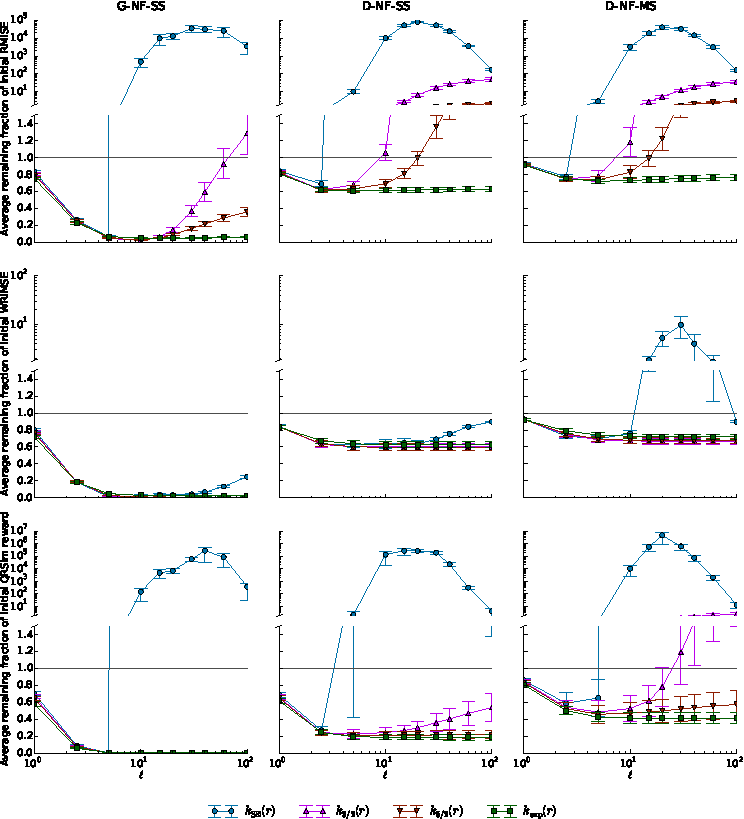
\includegraphics{plots/lengthscales}
    \caption[Influence of the length scale of the covariance functions]{The 
        normalized error for different covariance function in dependence of 
        length scale.  The rows correspond to the RMISE, WRMISE, and QRSim 
        reward error measures.  The columns correspond to a single source 
        Gaussian (G-NF-SS), a single source Gaussian dispersion (D-NF-SS), and 
        a multiple source Gaussian dispersion (D-NF-MS). All scenarios were 
        simulated without sensor noise.  Error bars represent the standard 
        error. The boundary of $1.0$ where the error of the trained Gaussian 
        process is larger than an all zero prediction is marked with 
        a horizontal line.}\label{fig:lengthscales}
\end{figure}

Comparing the WRMISE to the RMISE the former one stays quite low even for larger 
length scales. This indicates that in the area of the plume (also due to the more 
dense sampling) a good fit is still obtained, but around that area the 
prediction gets worse. Thus, the steep concentration gradients around the plume 
are not well captured in that case.

The results give also an idea how good of a fit can be expected at best when 
using an UAV\@. Whereas the normalized error decreases to nearly zero for the 
single source Gaussian, it stays above 0.6 for the dispersion scenario with the 
more localized plume distribution. The reward error measure is decreased to 
lower levels, but this is likely to underestimation of the error at the plume 
boundaries as argued in Chapter~\ref{sec:qrsim-reward}.

Besides the error measures the log likelihood of each trained Gaussian process 
was calculated. In Figure~\ref{fig:loglikelihood} the average over trials is 
plotted. Only for the squared exponential kernel the maximum of the log 
likelihood corresponds to the minimum of the RMISE\@. Towards longer length 
scales the likelihood declines very steeply. Using the log likelihood to 
estimate the length scales for the other covariance functions would largely 
overestimate it.

\begin{figure}
    \centering
    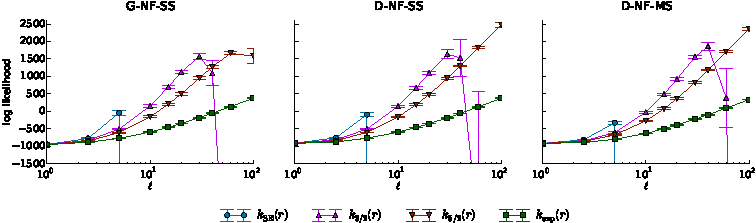
\includegraphics{plots/loglikelihood}
    \caption[Log likelihood in dependence of the kernel lengthscale]{The average 
        log likelihood of the training data in dependence of the length scale 
        using different kernels.  Each of the three plots shows one noise free 
        scenario of the single source Gaussian (G-NF-SS), single source Gaussian 
        dispersion (D-NF-SS), and multiple source Gaussian dispersion (D-NF-MS).  
        Error bars represent the standard error.}\label{fig:loglikelihood}
\end{figure}

Taken these results together it is best to choose a non-smooth kernel with 
a length scale of $\ell = \SI{5}{\meter}$. As it is advantageous to be able to 
use a gradient based optimizer for the optimization of acquisition functions, 
I decided to use the Matérn kernel with $\nu = 3/2$ in the further experiments, 
which gives a once mean square differentiable Gaussian process in opposite to 
the exponential kernel. Unfortunately, optimizing the length scale using the 
likelihood would not give good results and I fixed the length scale at $\ell 
= \SI{5}{\meter}$. Also, including a prior in the log likelihood does not help 
here. In example to shift the maximum of the likelihood for the chosen kernel to 
\SI{5}{\meter} a Gaussian prior would need a standard deviation of less then 
$\sigma_{\ell} < \e^{-2078} / \sqrt{2\uppi} \approx 0$ (see 
Apendix~\ref{sec:prior}).  Thus, effectively resulting in a fixed length scale.

\section{Comparison of Utility Functions}\label{sec:cmputility}
Given the kernel chosen in the previous section I continued to compare the 
different utility functions in the noiseless scenarios single source Gaussian 
(G-NF-SS-SV), single source dispersion (D-NF-SS-SV), and multiple source 
dispersion (D-NF-MS-SV).

For each given scenario 20~trials were performed. In each run the UAV first 
surrounded the simulation area in a height of \SI{40}{\meter} with a margin of 
\SI{10}{\meter} to the boundaries of the simulated volume. After that further 
way-points were chosen with one of the acquisition functions discussed in 
Chapter~\ref{sec:utility}. The optimization of that functions has been described 
in Chapter~\ref{sec:fnopt}.

Each trial was allowed to run until a maximum of \num{3000} plume measurements 
was acquired. A plume measurement was taken every second. When a new target 
way-point was within \SI{3}{\meter} of the previous one the UAV was considered 
to become stuck in a maximum of the acquisition function and the simulation was 
stopped at that point to reduce overall simulation time.

The error measures were estimated as described in Chapter~\ref{sec:error}. The 
samples for that where chosen from 1000 uniformly distributed sampling 
locations, every tenth of 4200 locations from the Metropolis-Hastings algorithm 
with Gaussian proposal distribution with standard deviation $\sigma 
= \SI{10}{\meter}$, and 10 more locations sampled from the proposal distribution 
for each of included Metropolis-Hastings samples.

I tested all three utility functions proposed in Chapter~\ref{sec:utility}: 
DUCB, PDUCB (with $\varepsilon = 10^{-30}$), and GO\@. DUCB was tested with 
a constant scaling factor of $s\ped{DUCB}(\vc y) = 1$ and the automatic scaling 
in Equation~\ref{eqn:scale-ducb}.  PDUCB was tested with a constant scaling 
factor of $s\ped{PDUCB}(\vc y) = 70$ (a little bit more than $-\ln \varepsilon$) 
and the automatic scaling in Equation~\ref{eqn:scale-pducb}.  Furthermore, 
I performed a parameter search over $\kappa \in \cbr{0.1, 0.5, 
0.75, 1, 1.25, 1.5, 2}$ and $\gamma \in \cbr{0} \cup \cbr{-10^p | p = -9, -8, 
  \dots, -2}$. Note that for the GO utility function the $\kappa$ parameter has 
no effect.

Figure~\ref{fig:psearch-G-NF-SS-SV}--\ref{fig:psearch-D-NF-MS-SV} visualize the 
normalized error for the different scenarios.  The respective parameters and 
values of the minima (excluding the QRSim reward) are listed in 
Table~\ref{tbl:err-g-nf-ss-sv}--\ref{tbl:err-d-nf-ms-sv}.  The average reduction 
(over trials) of the RMISE against simulation time in the single source Gaussian 
scenario (G-NF-SS-SV) is plotted in Figure~\ref{fig:errtrace-nf} and looks 
essentially the same for WRMISE and the QRSim reward and therefore it is not 
shown for those measures. Finally, Figure~\ref{fig:trajectory} visualizes an 
example UAV trajectory for the PDUCB acquisition function.

\begin{figure}
    \centering
    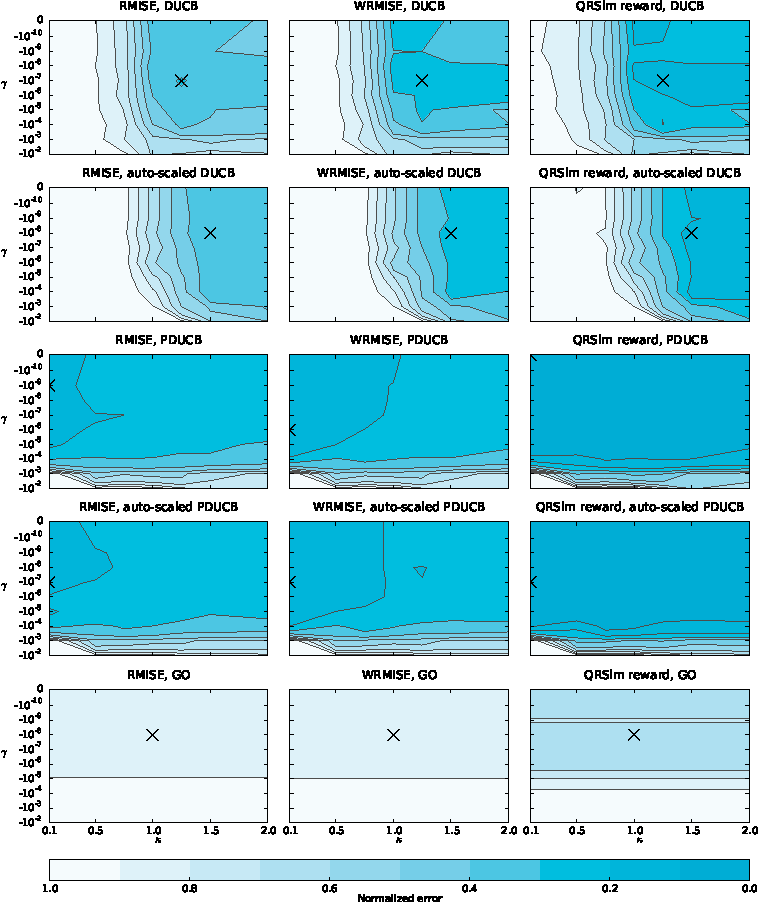
\includegraphics{plots/psearch-G-NF-SS-SV}
    \caption[Normalized error (G-NF-SS-SV)]{The normalized error for different 
        measures, utility functions, parameters in the noiseless single source 
        Gaussian scenario (G-NF-SS-SV).  The columns represent the RMISE, 
        WRMISE, and QRSim reward error measure.  The rows represent the DUCB, 
        auto-scaled DUCB, PDUCB, auto-scaled PDUCB and GO utility functions. The 
        auto-scaled versions use the scaling factor defined in 
        Equations~\ref{eqn:scale-ducb} and~\ref{eqn:scale-pducb}, in contrast to 
        a constant scaling factor. The minimum of each plot is marked with 
        cross.}\label{fig:psearch-G-NF-SS-SV}
\end{figure}

\begin{figure}
    \centering
    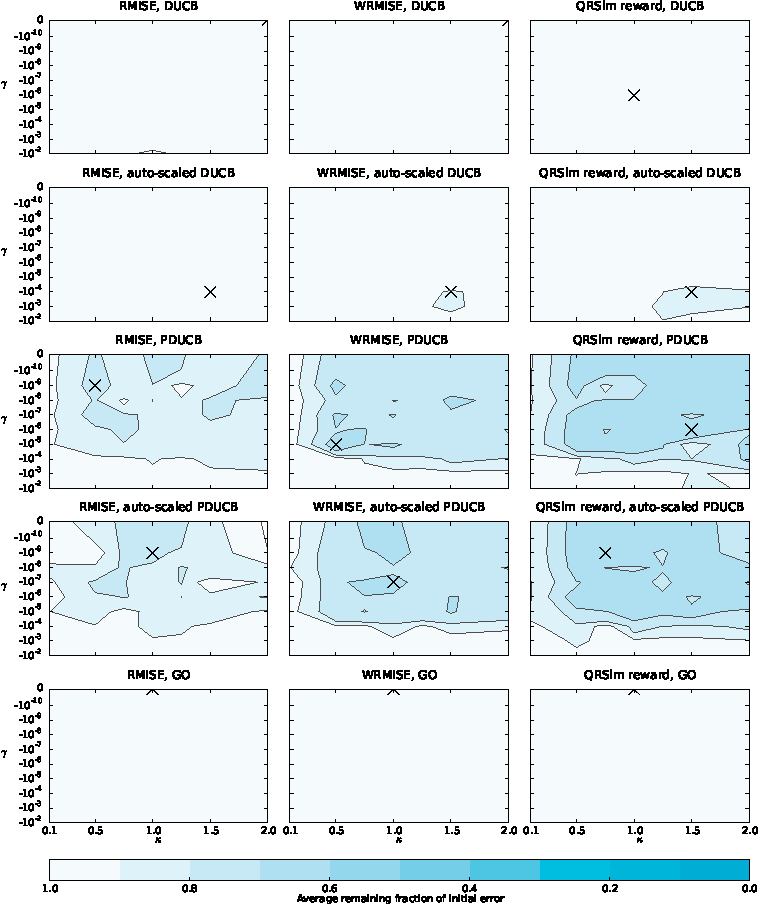
\includegraphics{plots/psearch-D-NF-SS-SV}
    \caption[Normalized error (D-NF-SS-SV)]{The normalized error for different 
        measures, utility functions, parameters in the noiseless single source 
        Gaussian dispersion scenario (D-NF-SS-SV).  The columns represent the 
        RMISE, WRMISE, and QRSim reward error measure.  The rows represent the 
        DUCB, auto-scaled DUCB, PDUCB, auto-scaled PDUCB and GO utility 
        functions. The auto-scaled versions use the scaling factor defined in 
        Equations~\ref{eqn:scale-ducb} and~\ref{eqn:scale-pducb}, in contrast to 
        a constant scaling factor.  The minimum of each plot is marked with 
        cross.}\label{fig:psearch-D-NF-SS-SV}
\end{figure}

\begin{figure}
    \centering
    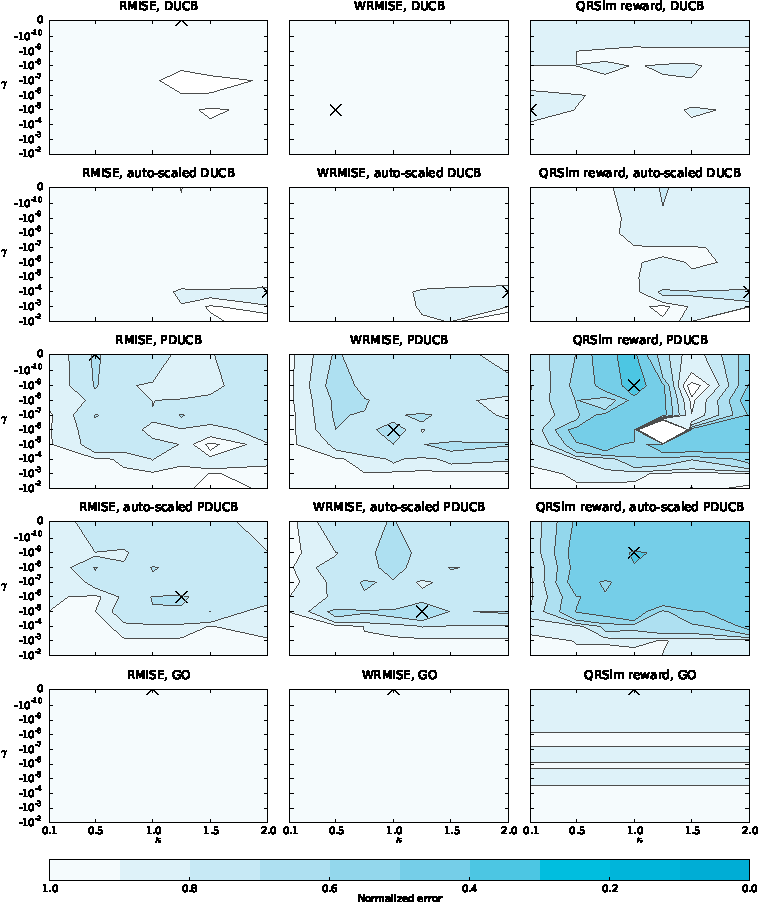
\includegraphics{plots/psearch-D-NF-MS-SV}
    \caption[Normalized error (D-NF-MS-SV)]{The normalized error for different 
        measures, utility functions, parameters in the noiseless multiple source 
        Gaussian dispersion scenario (D-NF-SS-SV).  The columns represent the 
        RMISE, WRMISE, and QRSim reward error measure.  The rows represent the 
        DUCB, auto-scaled DUCB, PDUCB, auto-scaled PDUCB and GO utility 
        functions. The auto-scaled versions use the scaling factor defined in 
        Equations~\ref{eqn:scale-ducb} and~\ref{eqn:scale-pducb}, in contrast to 
        a constant scaling factor.  The minimum of each plot is marked with 
        cross.}\label{fig:psearch-D-NF-MS-SV}
\end{figure}

\newenvironment{errtbl}{\begin{tabular}{lllSSSS}\toprule}{\bottomrule\end{tabular}}
\newcommand*{\errtblhead}[1]{
        & & &
        \multicolumn{2}{c}{#1} &
        \multicolumn{2}{c}{Norm.\ #1} \\
        \cmidrule(lr){4-5} \cmidrule(lr){6-7}

        Utility function &
        \multicolumn{1}{l}{$\kappa$} &
        \multicolumn{1}{l}{$\gamma$} &
        \multicolumn{1}{c}{Mean} &
        \multicolumn{1}{c}{SD} &
        \multicolumn{1}{c}{Mean} &
        \multicolumn{1}{c}{SD} \\
        & & &
        \multicolumn{1}{c}{\si{\nano\gram\per\meter\cubed}} &
        \multicolumn{1}{c}{\si{\nano\gram\per\meter\cubed}} &
        & \\ \midrule }

\begin{table}
    \centering
    \begin{errtbl}
        \errtblhead{RMISE}
        DUCB & 1.25 & \num{-1e-07} & 261.27 & 184.79 & 0.29 & 0.20 \\
        auto-scaled DUCB & 1.50 & \num{-1e-08} & 260.06 & 180.16 & 0.31 & 0.25 \\
        PDUCB & 0.10 & \num{-1e-09} & 206.79 & 242.72 & 0.18 & 0.13 \\
        auto-scaled PDUCB & 0.10 & \num{-1e-07} & 204.51 & 213.98 & 0.18 & 0.12 \\
        GO & 0.10 & \num{-1e-08} & 770.91 & 376.38 & 0.80 & 0.13 \\
        \midrule
        \\
        \errtblhead{WRMISE}
        DUCB & 1.25 & \num{-1e-07} & 121.46 & 122.79 & 0.21 & 0.22 \\
        auto-scaled DUCB & 1.50 & \num{-1e-08} & 127.55 & 123.92 & 0.25 & 0.28 \\
        PDUCB & 0.10 & \num{-1e-06} & 100.19 & 142.12 & 0.13 & 0.14 \\
        auto-scaled PDUCB & 0.10 & \num{-1e-07} & 100.58 & 137.84 & 0.13 & 0.13 \\
        GO & 0.10 & \num{-1e-08} & 489.22 & 258.44 & 0.80 & 0.15 \\
    \end{errtbl}
    \caption[Minimal error values G-NF-SS-SV.]{The minimal obtained error (RMISE 
        and WRMISE) for each acquisition function and the parameter values used 
        in the single source Gaussian scenario 
        (G-NF-SS-SV).}\label{tbl:err-g-nf-ss-sv}
\end{table}

\begin{table}
    \centering
    \begin{errtbl}
        \errtblhead{RMISE}
        DUCB & 2.00 & \num{0.0} & 5.33 & 3.90 & 0.94 & 0.10 \\
        auto-scaled DUCB & 1.50 & \num{-0.0001} & 5.00 & 3.67 & 0.91 & 0.16 \\
        PDUCB & 0.50 & \num{-1e-09} & 4.19 & 2.99 & 0.75 & 0.24 \\
        auto-scaled PDUCB & 1.00 & \num{-1e-09} & 4.10 & 2.85 & 0.76 & 0.24 \\
        GO & 0.10 & \num{0.0} & 5.40 & 3.88 & 0.95 & 0.09 \\
        \midrule
        \\
        \errtblhead{WRMISE}
        DUCB & 2.00 & \num{0.0} & 3.48 & 3.04 & 0.91 & 0.22 \\
        auto-scaled DUCB & 1.50 & \num{-0.0001} & 3.28 & 2.95 & 0.88 & 0.26 \\
        PDUCB & 0.50 & \num{-1e-05} & 2.29 & 2.20 & 0.63 & 0.39 \\
        auto-scaled PDUCB & 1.00 & \num{-1e-07} & 2.37 & 2.33 & 0.64 & 0.37 \\
        GO & 0.10 & \num{0.0} & 3.62 & 3.00 & 0.94 & 0.17 \\
    \end{errtbl}
    \caption[Minimal error values D-NF-SS-SV.]{The minimal obtained error (RMISE 
        and WRMISE) for each acquisition function and the parameter values used 
        in the single source Gaussian dispersion scenario 
        (D-NF-SS-SV).}\label{tbl:err-d-nf-ss-sv}
\end{table}

\begin{table}
    \centering
    \begin{errtbl}
        \errtblhead{RMISE}
        DUCB & 1.25 & \num{0.0} & 16.68 & 7.73 & 0.93 & 0.08 \\
        auto-scaled DUCB & 2.00 & \num{-0.0001} & 14.77 & 6.93 & 0.83 & 0.13 \\
        PDUCB & 0.50 & \num{0.0} & 13.13 & 7.82 & 0.68 & 0.18 \\
        auto-scaled PDUCB & 1.25 & \num{-1e-06} & 13.20 & 7.87 & 0.68 & 0.19 \\
        GO & 0.10 & \num{0.0} & 16.74 & 7.91 & 0.92 & 0.11 \\
        \midrule
        \\
        \errtblhead{WRMISE}
        DUCB & 0.50 & \num{-1e-05} & 11.35 & 6.58 & 0.93 & 0.14 \\
        auto-scaled DUCB & 2.00 & \num{-0.0001} & 9.66 & 6.11 & 0.80 & 0.21 \\
        PDUCB & 1.00 & \num{-1e-06} & 8.79 & 7.67 & 0.62 & 0.29 \\
        auto-scaled PDUCB & 1.25 & \num{-1e-05} & 8.44 & 7.02 & 0.65 & 0.26 \\
        GO & 0.10 & \num{0.0} & 11.30 & 6.48 & 0.93 & 0.12 \\
    \end{errtbl}
    \caption[Minimal error values D-NF-MS-SV.]{The minimal obtained error (RMISE 
        and WRMISE) for each acquisition function and the parameter values used 
        in the multiple source Gaussian dispersion scenario 
        (D-NF-MS-SV).}\label{tbl:err-d-nf-ms-sv}
\end{table}

\begin{figure}
    \centering
    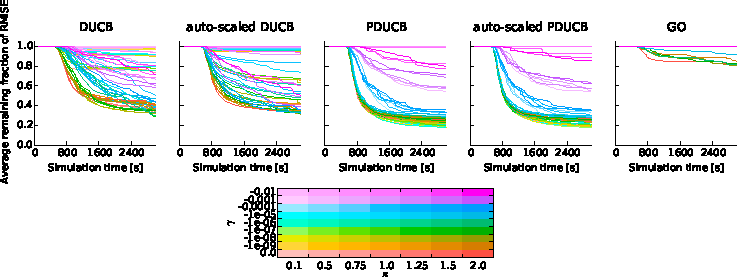
\includegraphics{plots/errtrace-nf}
    \caption[Time-course of the error reduction]{The normalized RMISE in the 
        single source Gaussian scenario (G-NF-SS-SV).  Each individual plot 
        corresponds to one utility function and scaling.  The auto-scaled 
        versions use the scaling factor defined in 
        Equations~\ref{eqn:scale-ducb} and~\ref{eqn:scale-pducb}, in contrast to 
        a constant scaling factor. The $\gamma$ parameter is coded by hue and 
        the $\kappa$ parameter by lightness.}\label{fig:errtrace-nf}
\end{figure}

\begin{figure}
    \centering
    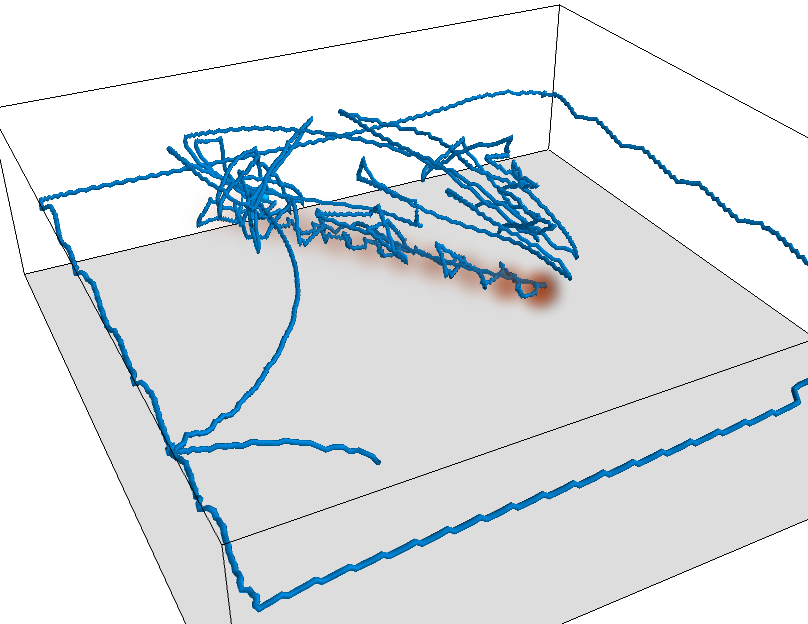
\includegraphics[width=6.5cm]{plots/trajectory}
    \caption[Example of an UAV trajectory]{Example of an UAV trajectory using 
        the PDUCB acquisition function with $\kappa = 1.25$, $\gamma 
        = -10^{-7}$, and automatic scaling in the single source Gaussian 
        scenario. The plume is shown in red.}\label{fig:trajectory}
\end{figure}

This is a rich dataset from which quite a few insights can be gained. First of 
all it can be noted that the normalized QRSim reward attributes almost always 
a better performance to the algorithms than the other two error measures.  This 
is consistent with the argument in Chapter~\ref{sec:qrsim-reward} that the 
reward may be underestimated at concentration boundaries.

Turning to the actual utility functions it can be noted that the GO function 
does not perform very well.  Even in the single source Gaussian scenario the 
RMISE is only reduced by about \SI{20}{\percent} and in the other two scenarios 
it performs even worse.

Comparing DUCB and PDUCB the latter one consistently performs better with 
a reduction in the RMISE and WRMISE by at least additional \SI{11}{\percent} and 
in the dispersion scenarios even more.  Despite that, the standard deviation of 
PDUCB is higher almost always higher than that of DUCB\@.

In the single source Gaussian scenario PDUCB proves to be quite robust against 
the choice of $\kappa$ as for all values very good results are obtained. This 
picture is a bit more noisy in the dispersion scenarios. It seems that too low 
values ($\kappa < 0.5$) degrade performance. This is consistent with the 
argument in Chapter~\ref{sec:utility} that a too low $\kappa$ limits the 
exploration and let the UAV become stuck in a (local) maximum. The choice of 
$\gamma$ has no considerable effect as long as the distance penalty is not 
chosen too large ($\gamma < -10^{-5}$).

The same behavior for the choice of $\gamma$ is also observed for DUCB in the 
single source Gaussian scenario. However, this utility function is far more 
sensitive to the choice of $\kappa$. Using the scaling $s\ped{DUCB}(\vc y) = 1$ 
the performance degrades setting $\kappa < 1$ and using the automatic scaling it 
degrades for $\kappa < 1.5$. In the dispersion scenarios the DUCB acquisition 
function does not perform well for any tested combination of parameter values.

Interestingly,  DUCB performs slightly better with automatic scaling, whereas 
PDUCB performs slightly worse.

Finally, taking a look at the time course of error reduction multiple phases can 
be discovered where a reasonable reduction of the error occurs. About the first 
\SI{500}{\second} nearly no reduction occurs as in this phase the UAV only 
surround the area of interest. Then the error rapidly decreases in the next 
\SIrange{1000}{2000}{\second} until the decrease levels off and stays fairly 
constant for the rest of the simulation time.

These results show that PDUCB outperforms the DUCB and GO acquisition functions 
and in addition is quite robust against a non-optimal choice of parameters. The 
especially bad performance of the GO utility function is not too surprising at 
its intended use is to find a function maximum and not building a correct model 
of the function (respectively plume concentration).  DUCB works reasonable well 
for the simple case of a Gaussian distribution, but fails for the more localized 
dispersions.

The PDUCB performance might not seem to be too impressive in the dispersion 
scenarios, too. However, one has to keep in mind that even in 
Section~\ref{sec:bestkernel} with much more samples the RMISE could not be 
reduced to less than \SI{61}{\percent}.  Also, the qualitatively the plume is 
predicted at the correct location as Figure~\ref{fig:plume} shows, despite some 
deviance of the exact concentration values. The largest difference to the true 
distribution is close to the source at the concentration maximum.

\begin{figure}
    \centering
    \subfigure[Prediction]{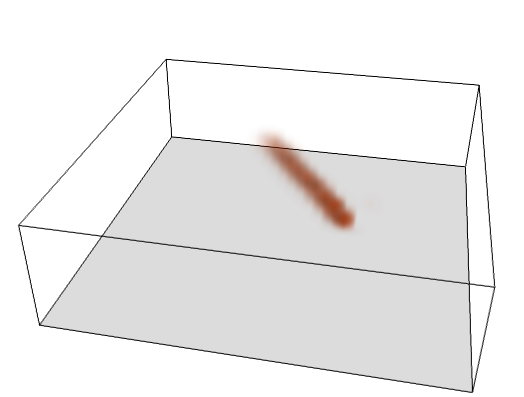
\includegraphics[width=0.3\textwidth]{plots/plume-prediction}\label{fig:plume-prediction}}
    \subfigure[Difference]{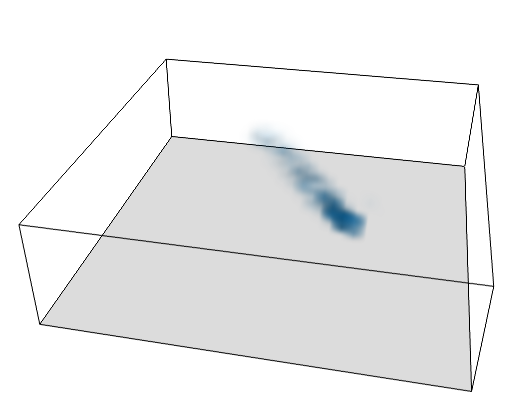
\includegraphics[width=0.3\textwidth]{plots/plume-diff}\label{fig:plume-diff}}
    \subfigure[True 
    distribution]{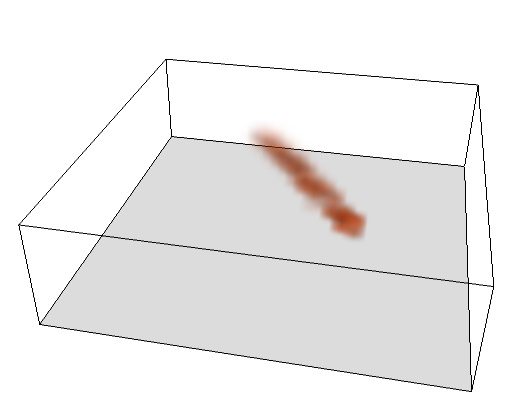
\includegraphics[width=0.3\textwidth]{plots/plume-true}\label{fig:plume-true}}
    \caption[Example visualization of the plume prediction]{One instance of the 
        single source Gaussian dispersion scenario (D-NF-SS-SV).  
        \subref{fig:plume-prediction} Mean of the Gaussian process.  
        \subref{fig:plume-diff} The absolute value of the difference of the 
        predicted and true distribution.  \subref{fig:plume-true} The true plume 
        distribution.}\label{fig:plume}
\end{figure}

Given this discussion I decided to limit further experiments to the PDUCB 
acquisition function as the other options seem to not a viable option (except 
maybe for the single source Gaussian). As smaller values of $\kappa$ seem to 
provide slightly better results, but it should not be below $1$ as argued, 
a value of $\kappa = 1.25$ was selected. The penalty distance seems to slightly 
improve the results up to \num{-1e-5}. However, to prevent to fall in the area 
where the performs then quickly decreases, it was set to a lower value of 
$\gamma = \num{-1e-7}$ which also good results. Both scaling approaches 
(constant or automatic) where used in further experiments as it is not clear 
from these results which one is better. Though, the automatic scaling is a bit 
worse in terms of error, it has one less parameter which would be set according 
to the range of concentration values.

\section{Evaluation in a Noisy Setting}\label{sec:noisy}
It is important to verify that the methods for plume modelling also work in 
a noisy environment as in the real world noise will necessarily occur. For that 
a standard deviation of the sensor noise of $\sigma\ped{noise} 
= \SI{1e-5}{\gram\per\meter\cubed}$ was assumed. As it should be possible to 
reliably estimate the noise level of the sensor, I considered this value as 
known. That allows to set the noise variance of the Gaussian process 
$\sigma\ped{n}^2 = \sigma\ped{noise}^2$. For a good prediction the ratio of 
$\sigma\ped{n}^2$ and the kernel variance $\sigma\ped{k}^2$ has to be chosen 
well. The process of doing that will be discussed in the next section before 
returning to the actual simulations.

\subsection{Choosing the Kernel Variance}
The method for determining the kernel variance was essentially the same as 
described in Section~\ref{sec:bestkernel} for determining the length scale. The 
points were it differs are that instead of the noiseless scenarios the single 
and multiple source plume dispersion scenarios with sensor noise (D-SN-SS-SV, 
D-SN-MS-SV) were used and only the Mat\'ern kernel with $\nu = 3/2$ was used.  
Instead of varying the length scale it was fixed to $\ell = \SI{5}{\meter}$ and 
the kernel variance $\sigma\ped{k}^2$ was varied from 
\SIrange{1e-12}{1e-3}{\gram\squared\per\meter\tothe{6}}.

The results are shown in Figure~\ref{fig:kvar}. The normalized error measures 
are highest for low values of $\sigma\ped{k}^2$ approaching 1. For 
$\sigma\ped{k}^2 > \SI{1e-9}{\gram\squared\per\meter\tothe{6}}$ the WRMISE stays 
the same, but the RMISE and QRSim reward slightly increase. This is even less 
pronounced for multiple sources.

\begin{figure}
    \centering
    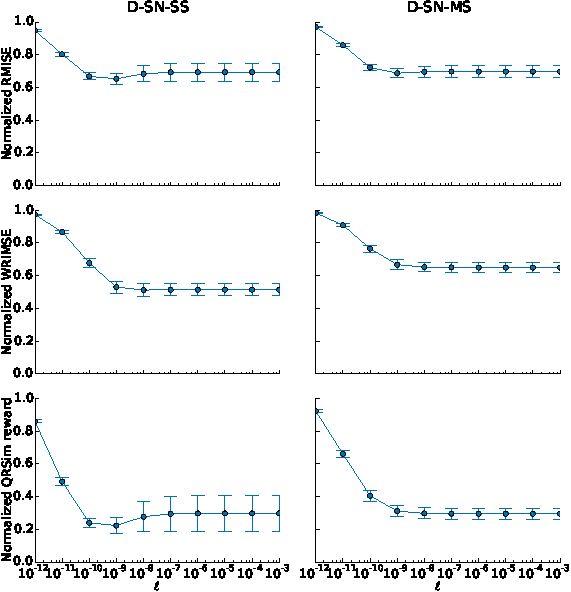
\includegraphics{plots/kvar}
    \caption[Influence of the kernel variance]{The normalized error using the 
        Mat\'ern kernel ($\nu = 3/2$) in dependence of the kernel variance..  
        The rows correspond to the RMISE, WRMISE, and QRSim reward error 
        measures.  The columns correspond to a single source Gaussian (G-SN-SS), 
        and a single source Gaussian dispersion (D-SN-SS). Both scenarios were 
        simulated with sensor noise.  Error bars represent the standard 
        error.}\label{fig:kvar}
\end{figure}

As all error measures do have their minimum at $\sigma\ped{k}^2 
= \SI{1e-9}{\gram\squared\per\meter\tothe{6}}$ or have almost reached it, this 
value has been used in the following.

\subsection{Simulation of the Scenarios Including Noise}
Using the kernel variance of $\sigma\ped{k}^2 
= \SI{1e-9}{\gram\squared\per\meter\tothe{6}}$ determined in the previous 
section the PDUCB method was evaluated in the single and multiple source plume 
dispersion scenario including sensor noise (D-SN-SS-SV, D-SN-MS-SV). The sensor 
noise variance and the noise variance of the Gaussian process were set to 
$\sigma\ped{noise}^2 = \sigma\ped{n}^2 
= \SI{1e-10}{\gram\squared\per\meter\tothe{6}}$.  As the change of 
$\sigma\ped{k}^2$ (previously set to 1) influences $\sigma^2(\vc x)$ the value 
of $\kappa$ has to be adjusted by the inverse factor. Hence, the PDUCB parameter 
setting in the following were $\kappa = \num{1.25e9}$ and $\gamma 
= \num{-1e-7}$.

In many instances surrounding the simulation area in just one height is not 
sufficient to discover the plume under the influence of noise. Thus, the 
complete search and the wind based search strategy described in 
Chapter~\ref{sec:bootstrapping} have been employed. The latter approach requires 
of course wind information which was read out from the QRSim simulator.

Apart from these points the same methods as in the noiseless case 
(Section~\ref{sec:cmputility}) were used including the same number of 20~trials.

The results are shown in Figure~\ref{fig:noisy-ss} and Tables~\ref{tbl:noisy-ss} 
and~\ref{tbl:noisy-ms}. All tested variants reduce the normalized RMISE to 
a value between \numrange{0.70}{0.83} in both scenarios with a similar standard 
deviation around \numrange{0.17}{0.24} in the single source scenario.  Using the 
wind based search the error starts to decrease earlier in the single source 
scenario as less area has to be covered.  Also the overall decrease seems to be 
a bit faster after the plume has bee discovered.

\begin{figure}
    \centering
    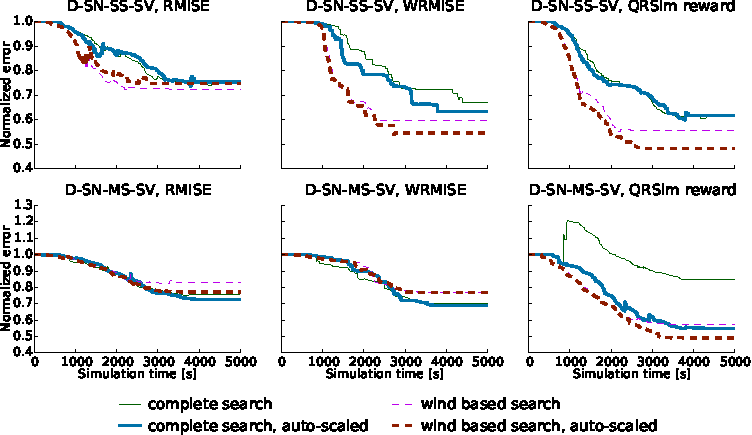
\includegraphics{plots/noisy-sv}
    \caption[Normalized error in scenarios with sensor noise]{Average normalized 
        error over time in the single source dispersion (D-SN-SS-SV, top row) 
        and multiple source dispersion scenario (D-SN-MS-SV, bottom row). Both 
        including sensor noise.  The columns columns correspond to the RMISE, 
        WRMISE and the QRSim reward as error meausure. Solid lines show the 
        results using the complete search method, where as dashed lines used the 
        wind based search.  Thick lines show PDUCB with automatic scaling 
        opposed to a constant scaling shown by the thin 
        lines.}\label{fig:noisy-ss}
\end{figure}

\newenvironment{errtblb}{\begin{tabular}{llSSSS}\toprule}{\bottomrule\end{tabular}}
\newcommand*{\errtblheadb}[1]{
        & &
        \multicolumn{2}{c}{#1} &
        \multicolumn{2}{c}{Norm.\ #1} \\
        \cmidrule(lr){3-4} \cmidrule(lr){5-6}

        Search method &
        \multicolumn{1}{l}{Scaling} &
        \multicolumn{1}{c}{Mean} &
        \multicolumn{1}{c}{SD} &
        \multicolumn{1}{c}{Mean} &
        \multicolumn{1}{c}{SD} \\
        & &
        \multicolumn{1}{c}{\si{\nano\gram\per\meter\cubed}} &
        \multicolumn{1}{c}{\si{\nano\gram\per\meter\cubed}} &
        & \\ \midrule }

\begin{table}
    \centering
    \begin{errtblb}
        \errtblheadb{RMISE}
        complete & constant & 4.06 & 2.60 & 0.75 & 0.24 \\
        complete & auto & 4.16 & 2.83 & 0.75 & 0.23 \\
        wind & constant & 3.90 & 2.43 & 0.72 & 0.21 \\
        wind & auto & 3.95 & 2.69 & 0.75 & 0.23 \\
        \midrule
        \\
        \errtblheadb{WRMISE}
        complete & constant & 2.57 & 2.26 & 0.67 & 0.32 \\
        complete & auto & 2.55 & 2.63 & 0.63 & 0.36 \\
        wind & constant & 2.27 & 2.05 & 0.60 & 0.33 \\
        wind & auto & 1.85 & 1.66 & 0.55 & 0.32 \\
    \end{errtblb}
    \caption[Final error values D-SN-SS-SV]{Final error values in the noisy 
        single source Gaussian scenario (D-SN-SS-SV).}\label{tbl:noisy-ss}
\end{table}

\begin{table}
    \centering
    \begin{errtblb}
        \errtblheadb{RMISE}
        complete & constant & 14.07 & 8.16 & 0.75 & 0.21 \\
        complete & auto & 13.53 & 7.51 & 0.73 & 0.17 \\
        wind & constant & 15.68 & 8.72 & 0.83 & 0.22 \\
        wind & auto & 14.75 & 8.33 & 0.77 & 0.22 \\
        \midrule
        \\
        \errtblheadb{WRMISE}
        complete & constant & 9.02 & 7.36 & 0.70 & 0.29 \\
        complete & auto & 13.53 & 7.51 & 0.73 & 0.17 \\
        wind & constant & 9.99 & 6.96 & 0.77 & 0.24 \\
        wind & auto & 14.75 & 8.33 & 0.77 & 0.22 \\
    \end{errtblb}
    \caption[Final error values D-SN-MS-SV]{Final error values in the noisy 
        multiple source Gaussian scenario (D-SN-MS-SV).}\label{tbl:noisy-ms}
\end{table}

Looking at the WRMISE for a single source it turns out that the wind based 
search decreases the normalized error by about \SI{7}{\percent} additionally 
compared to the complete search. Thus, the wind based search is able to better 
approximate the actual plume without increasing the approximation error in other 
areas. With regard to the WRMISE the automatic scaling seems to perform a bit 
better (difference of \num{0.05} in the normalized error), but this is not the 
case for the RMISE\@. Given multiple source the performance of the search 
strategies is almost equal.  Also, the scaling method does not have 
a significant influence.

In the QRSim reward estimation occurs again an artifact in the multiple source 
scaling as already seen in Section~\ref{sec:cmputility}.

The results show that PDUCB can also be applied in a noisy setting. In 
comparison to a noiseless setting the error in the estimation slightly increases 
as would be expected given the same amount of training samples. However a more 
extensive search strategy has to applied in the beginning. Using wind 
information a good estimation might be obtained more quickly, but the effect is 
rather small if existent at all. Both, a constant scaling and the automatic 
scaling perform equally. This makes the automatic scaling a better choice as it 
requires to set less parameters.

\section{Multiple UAVs}
Finally, the performance of the PDUCB acquisition function with the extension 
for multiples UAVs (Chapter~\ref{sec:multiple-uavs}) has been evaluated. For 
this exactly the same methods as in the previous section were used with 
exception of the scenario. This was replaced by the multiple UAV, multiple 
source plume dispersion scenario (D-SN-MS-MV). Also, a number of different $\rho 
\in \{10^{-i} | i = 5, \dots, 11\}$ has been tested.

Figure~\ref{fig:mv-err} shows the final normalized error in dependence of the 
value of $\rho$. Unfortunately, it is not possible to identify one value which 
is clearly better than others. Also, the normalized error is seldom decreased 
below \num{0.8}. The best result is still obtained by the wind based search with 
auto-scaled PDUCB\@. This is most prominent for the WRMISE\@.

\begin{figure}
    \centering
    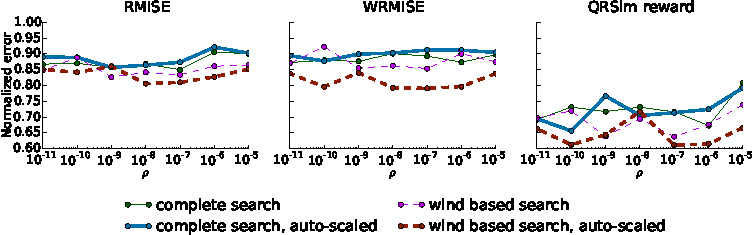
\includegraphics{plots/multiple-uav}
    \caption[Normalized error using multiple UAVs]{The final normalized error 
        using multiple UAVs in the multiple source scenario (D-SN-MS-MV). Each 
        plot corresponds to a different error measure.Solid lines show the 
        results using the complete search method, where as dashed lines used the 
        wind based search.  Thick lines show PDUCB with automatic scaling 
        opposed to a constant scaling shown by the thin 
        lines.}\label{fig:mv-err}
\end{figure}

To understand why the performance of multiple UAVs is at best the same as of 
a single one it helps to directly compare those two scenarios as done in 
Figure~\ref{fig:sv-vs-mv}. The decrease of the error stops earlier with multiple 
UAVs as the limit of training samples is faster reached with more UAVs sampling.  
As the error is decreasing only slightly faster with multiple UAVs the 
additional UAVs acquire samples in regions which do not add much to the overall 
estimation of the plume.

There are different reasons why that might be the case. The plume of a single 
source has a small spatial extent (except along the wind direction). Only one 
UAV can acquire samples in it without risking a collision with other UAVs.  
Moreover, the initial search strategy might be a problem. After one plume has 
been identified all vehicles switch to using the acquisition function. However, 
this makes the discovery of further plumes somewhat random.

In conclusion there is definitely room for improvement regarding the usage of 
multiple UAVs.

\begin{figure}
    \centering
    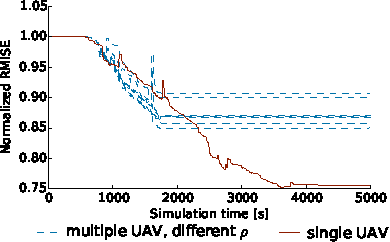
\includegraphics{plots/sv-vs-mv}
    \caption[Comparing the usage of a single and multiple UAVs.]{Comparison of 
        the average normalized RMISE over time for a single UAV (solid line) and 
        multiple UAVs (dashed lines, each line is a different $\rho$). In both 
        setting a total of \num{3000} samples was acquired.}\label{fig:sv-vs-mv}
\end{figure}
